% Plantilla para Artículos Científicos en LaTeX - CyTA
% Basado en la plantilla original con mejoras para integración con GitHub y curación semántica

\documentclass[a4paper,12pt]{article}
\usepackage[utf8]{inputenc}
\usepackage[T1]{fontenc}
\usepackage{graphicx}
\usepackage{float}
\usepackage{hyperref}
% Paquete para referencias en formato APA
\usepackage[style=apa,sorting=nyt]{biblatex}
\addbibresource{references.bib} 
% Archivo .bib con las referencias
\usepackage{lmodern}
\usepackage{geometry}
\geometry{margin=1in}
\usepackage{amsmath, amssymb, amsfonts}
\usepackage{listings} % Para código fuente

% Metadatos RDFa y Schema.org en LaTeX
\hypersetup{
pdfauthor={Nombre del Autor},
pdftitle={Título del Artículo},
pdfsubject={Disciplina científica},
pdfkeywords={Palabras clave, CyTA, Web Semántica},
pdfproducer={LaTeX con BibTeX},
pdfcreator={pdfLaTeX}
}

% Cargar metadatos desde archivo externo
% metadata.tex - Metadatos para artículos en LaTeX con RDFa/Schema.org

% Título y autores
\title{Título del artículo en LaTeX con Metadatos Semánticos}  
\author{Nombre del Autor\thanks{ORCID: 0000-0000-0000-0000, Afiliación}}  
\date{\today}  

% Palabras clave
\keywords{Palabra clave 1, Palabra clave 2, Palabra clave 3}  

% Licencia Creative Commons
\usepackage{ccicons}
\newcommand{\licencia}{\ccby \ccnc \ccsa}

% Metadatos RDFa / Schema.org
\usepackage{xmpincl} % Para incluir metadatos en PDF
\includexmp{metadata} % Archivo RDF/XML externo con datos estructurados


\title{\textbf{Título del Artículo Científico}}

\author{
Autor Uno $^{1,}$ \\
\small $^1$ Afiliación 1, Ciudad, País \\
\small ORCID: \texttt{0000-0000-0000-0000} \\
\small \texttt{email1@ejemplo.com} 
\and
Autor Dos $^{2,}$ \\
\small $^2$ Afiliación 2, Ciudad, País \\
\small ORCID: \texttt{0000-0000-0000-0000} \\
\small \texttt{email2@ejemplo.com} 
\and
Autor Tres $^{3,}$\\
\small $^3$ Afiliación 3, Ciudad, País \\
\small ORCID: \texttt{0000-0000-0000-0000} \\
\small \texttt{email3@ejemplo.com} 
}




\date{\today}


% Metadatos semánticos RDFa/Schema.org
% @context: https://schema.org
% @type: ScholarlyArticle
% headline: \documentTitle
% author: \authorName
% datePublished: \today
% publisher: CyTA

\begin{document}

\maketitle

\begin{abstract}
\textbf{Purpose} - Rapid response is often the cornerstone of success in many industries, especially manufacturing. In the authors’ opinion, organizational structure will also affect the construction of a fast-response supply chain system. The main purpose of this research examines whether different levels of organizational structure have different effects on the relationship between external integration and firm performance. 

 \textbf{Design/Methodology/Approach} - This study applied questionnaires to collect data. This study collected 818 questionnaires from manufacturers in China, Hong Kong and Taiwan to verify our proposed model using structural equation modeling.

\textbf{Findings} - Results show that response speed perfectly mediates the relationship between external integration and firm performance. Different levels of organizational structure will also affect external integration. Strict organizational structure requires customer integration, while loose organizational structure requires supplier integration to quickly meet customer needs.

\textbf{Practical implications} - Companies can probably determine whether their organizational structure is higher or lower than that of their competitors. If firms can determine that their organization structure is high or low, they can adopt suitable external integrations to enhance quick response and operational performance.

\textbf{Originality/Value} - In the relationship between supply chain integration and performance, we consider a mediating variable and moderating variable together. Results explain the reason that the relationship between supply chain integration and performance are inconsistent in previous studies. We have addressed external integration in alignment with organizational structure to provide better service and enhance performance by providing empirical evidence.

\href{https://www.cyta.com.ar/biblioteca/bddoc/bdlibros/ciencia_alto_impacto.htm#x5-3}{Ver referencias}

\textbf{Keywords:} keyword 1; keyword 2; keyword 3, keyword 4; keyword 5

\end{abstract}

\newpage
\section*{Template Overview}

\begin{figure}[h]
    \centering
    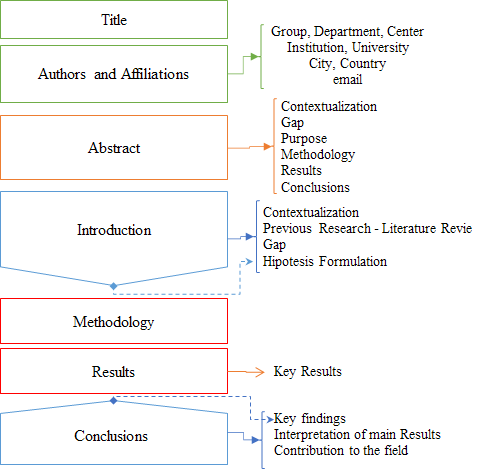
\includegraphics[width=0.9\linewidth]{Figures/article.png}
    \caption{Aartículo científico: esquema para su elaboración}

   \label{fig:article}
\end{figure}
\textbf{Para más información, sobre la estructura y la correcta escritura en cada seción  del artículo, consulte los siguientes textos: 
}
\begin{itemize}
    \item \href{https://www.cyta.com.ar/biblioteca/scientific_publications/scientific_writing.html}{Scientific writing},\parencite{scientific_writing} y 
    \item \href{https://www.cyta.com.ar/biblioteca/bddoc/bdlibros/ciencia_alto_impacto.htm#x5-1}{Ciencia de alto impacto, en particular el punto 5.1 Organización de un texto científico} \textcite{ciencia_alto_impacto}
   \item 
   También puede consultar a ChatGPT, indicando la refrencia de CyTA
\cite{chatgpt2025rdf}
\end{itemize}

\newpage
\section{Título, Autor, Afiliación}
\label{sec:Title,Creator}

\subsection{Título}

El título es una etiqueta y tiene que describir precisamente el contenido del artículo.
\vspace{5mm} %5mm vertical space

\textit{Función}:

\begin{itemize}
    \item Atraer la atención del lector.
    \item Describir el contenido del artículo.
    \item Enfatizar los hallazgos clave.
    \item Utilice el mínimo número de palabras.
\end{itemize}
\vspace{5mm} %5mm vertical space

\textit{Reglas}:

\begin{itemize}
    \item Conciso y claro .
    \item Aplicar palabras específicas asociadas al resultado del trabajo
    \item Longitud promedio: 14 palabras.
    \item Sin siglas ni abreviaturas, excepto aquellas que toda la audiencia conoce.
    \item Ningún título llevará punto final.
\end{itemize}
\vspace{5mm} %5mm vertical space

\textit{Sugerencia}: reescribir el título en la versión final del artículo. 

\subsection{Autores y Afiliación}

\begin{itemize}
    \item \textit{Pauta para definir la autoría}: Todos los autores deben poder presentar, discutir y defender el artículo.
    \item \textit{Secuencia de nombres de los autores}: Nombre-Segundo nombre-Apellido.
    \item \textit{Las afiliaciones generalmente incluyen la siguiente información}: Grupo; Departamento, Centro, Universidad; Institución; Ciudad; País.
    \item \textit{email}: Se deben proporcionar las direcciones de correo electrónico de todos los autores, para generar un contacto directo.
\end{itemize}

\section{Resumen (Abstract)}

El resumen debe exponer secuencialmente de forma encadenada, la importancia de la línea de investigación realizada y contextualizada en un campo de conocimiento; las evidencias relevantes que valorizan el por qué se realiza el estudio (antecedentes) ; el propósito (objetivo) sustentado en un claro planteo del problema; seguidamente, se exponen los métodos utilizados; luego los resultados o principal hallazgo en función del objetivo planteado; y finalmente, la conclusión de cómo los resultados aportan al campo disciplinar de la investigación.

\subsection{Tipos}


\begin{itemize}
    \item Informativo: Contiene toda la información relevante del trabajo.
    \item Descriptivo: Describe únicamente la naturaleza o el propósito del estudio.
\end{itemize}

\subsection{structura del resumen}

\begin{enumerate}
    \item Contextualización / Antecedentes;
    \item Brecha;
    \item Propósito / Objetivos;
    \item Metodología;
    \item Resultados;
    \item Conclusión.
\end{enumerate}
Si los autores son investigadores experimentados, y con buena capacidad de construcción semántica, la estructura de sus resúmenes podrá estar compuesta por cuatro enunciados: 

\begin{enumerate}
    \item Propósito / Objetivos;
    \item Metodología;
    \item Resultados;
    \item Conclusión.
\end{enumerate}

\subsection{Estilo gramatical}

Preferentemente utilice:

\begin{itemize}
    \item \textit{la voz activa (sujeto, predicado, objeto)}: para crear oraciones directas, claras y concisas, especialmente cuando esté escribiendo sobre las acciones de personas (los niños comieron las galletas); y
    \item \textit{la voz pasiva (}\textit{objeto, predicado, sujeto}\textit{)}: cuando sea más importante centrarse en el objeto destinatario de una acción, como al describir una configuración experimental (las galletas fueron comidas por los niños).
\end{itemize}
\href{https://apastyle.apa.org/style-grammar-guidelines/grammar/active-passive-voice}{https://apastyle.apa.org/style-grammar-guidelines/grammar/active-passive-voice}

\section{Palabras Clave (Keywords)}

\begin{itemize}
    \item Cantidad de palabras claves sugeridas: entre 3 (tres) y 5 (cinco);
    \item Escribirlas separadas por coma y sin punto final;
    \item Elija términos específicos, genéricos y relacionados del tesauro de la  (\href{https://vocabularies.unesco.org/browser/thesaurus/en/}{UNESCO}), o algún tesauros específico del campo disciplinar.
\end{itemize}
\newpage
\section{Introducción}
\subsection{Arquitectura de la 
{\textit{Información}}: }
\begin{enumerate}
    \item Contextualización / Estado del arte /: ¿por qué es importante esta área?; ¿qué se ha hecho antes? →Revisión de la literatura científica: artículos seminales, artículos recientes;
    \item Brecha: Lo que no se ha hecho →Revisión de la literatura científica: Artículos más recientes;
    \item Propósito / Relevancia / Motivación / Importancia: ¿Por qué es importante este estudio?, ¿Qué se presenta aquí? → Revisión de la literatura científica: Artículos seminales, Artículos más recientes → Formulación de hipótesis.
\end{enumerate}

\begin{figure}[hbt!]
    \centering   
    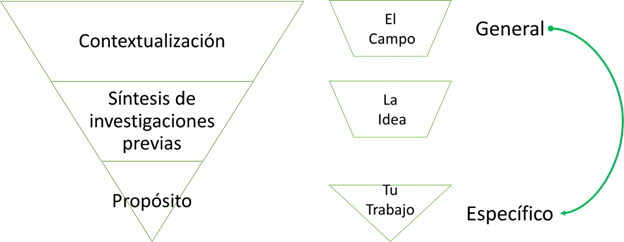
\includegraphics[width=0.9\linewidth]{Figures/imagen16_article_informacion.png
}
    \caption{Structure of the information}
    \label{fig:Structure of the information}
\end{figure}

\textbf{
\subsection{Estilo}
}
\begin{itemize}
    \item Contextualización y Gap: Generalmente se utiliza pasado, presente perfecto (continuo).
    \item Propósito: Es preferible el tiempo presente o pasado.
    \item Utilice la voz activa tanto como sea posible.
    \item Tercera persona con algún uso de primera persona.
\end{itemize}
\section{Metodología}
\textit{Methods} En principio se debe tener presente las teorías o leyes que delimitaron la hipótesis o el planteo del problema, que conlleva un resultado a priri esperado congruente con el objetivo, todo expresado en la introducción, y que han de establecer consecuentemente el tipo de metodología que se aplica para resolver el problema de investigación.

Entonces, no sólo se expone cómo se aplicaron los mejores medios para alcanzar los fines preexistentes; también debe permitir aprender, mediante los resultados alcanzados y la discusión a ser expuestos, a aumentar el conocimiento.

\section{Resultados, Discusión, Conclusión}
\label{sec:Results,Discussion,Conclusion}
 
 Posibles estructuras:

\begin{itemize}
    \item Resultados / Discusión / Conclusión
    \item Resultados y Discusión / Conclusión
    \item Resultados / Discusión y Conclusión
\end{itemize}
 
\subsection{Resultados y discusión}
Es la sección más importante de un artículo, en ella es donde  se prueba la pregunta inicial del problema, o mejor ahún la hipótesis. 
Se representan a traves de materiales ilustrativos (figuras, tablas, gráficos, imágenes), y principalmente a través de  cálculos y con un texo que atienda a una semántica bien constituida.

La forma en que se redactan los logros hace toda la diferencia, de ahí la importancia de la calidad de las figuras, el análisis de datos y el rigor estocástico.

\subsubsection{Modelo sugerido}
\begin{itemize}
    \item Antecedentes / Importancia
    \item Describe los resultados de la investigación (figuras, tablas, gráficos, imágenes, cálculos, pruebas de algoritmos, etc.)
    \item Interpretación
    \item Comparación
    \item Trascendencia
\end{itemize}
 
\subsubsection{Estilo}

\begin{itemize}
    \item Tiempo pasado;
    \item Tercera Persona, preferiblemente;
    \item Utilice la voz activa siempre que sea posible;
    \item Los subtítulos pueden mejorar la organización y la comprensión.
\end{itemize}

Lograr un equilibrio entre la descripción de los datos en el texto y en la leyenda de la figura/tabla

Todo lector debe comprender una figura/tabla sin leer la sección de resultados.

Numeración: Las figuras y tablas se numeran independientemente.

Abreviatura:

“Figura” puede abreviarse como “Fig.” en el texto, pero no en la leyenda.

“Tabla” no se abrevia.

Consulte siempre la Guía para autores de la revista.

El lugar adecuado para los subtítulos

Tablas: arriba, justificadas a la izquierda.

Figuras: abajo, justificadas a la izquierda

Lograr un equilibrio entre la descripción de los datos en el texto y en la leyenda de la figura/tabla

Cualquier lector debe comprender una figura/tabla sin leer la sección de resultados.

Consejos

Subtítulos

Las leyendas deben transmitir la mayor cantidad de información posible: los sujetos del experimento, la relación mostrada, los tamaños de muestra y las pruebas estadísticas si no se muestran en otro lugar.

¿Realmente necesitas una figura?

“El espesor de la película se estimó en 10 nm por bicapa, utilizando AFM….”

“La producción de semillas fue mayor para las plantas en el tratamiento de pleno sol (52,3 +/- 6,8 semillas) que para las que recibieron luz filtrada (14,7 +/- 3,2 semillas)….”

Nota: Utilice siempre un espacio entre el valor y la unidad:

“La longitud estimada fue de 10 m”, o bien, “el tiempo óptimo fue de 100 min”.

\subsection{Conclusiones}

Su principal función es la de exponer la importancia del artículo para el desarrollo del campo disciplinar al cual pertenece la investigación.

Las ideas racional han de fluir  de lo específico, que surge del principal resultado, a  lo general que es el encuadre en el marco teórico correspondiente, por el cual son interpretados los resultados y su correspondiente aporte al conocimiento cintífico. Esta estructura piramidal puede representarse en la siguiente figura:

\begin{figure}[hbt!]
    \centering
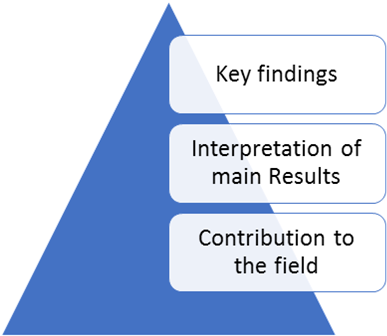
\includegraphics[width=0.5\linewidth]{Figures/article_conclusion.png}
    \caption{Conclusion structure}

    \label{fig:conclusion}
\end{figure}


\subsubsection{Modelo sugerido}

\begin{itemize}
    \item Enuncie los principales hallazgos: enfatice sus principales resultados.
    \item Interpretación de los principales hallazgos: tome unas cuantas frases para reformular la interpretación de los resultados clave.
    \item Contribuciones/Progresos en el campo: Describa las implicaciones de sus logros en el campo.
\end{itemize}

\subsubsection{Estilo}
\begin{itemize} 
    \item Tiempo pasado y presente;
    \item  Tercera Persona, preferentemente.
    
\end{itemize} 


\printbibliography % Imprime las referencias automáticamente desde el archivo .bib

\newpage
\section{Tablas, Figuras, y Escritura matemática }
\label{sec:tablas_figuras_matematic}

\subsection{Tablas}
Las tablas se numeran en forma ascendente y el título se coloca en la parte superior de la misma, escribiendo con letras minúsculas salvo el primer literal del primer término o nombres propios; ejemplo de Tabla:

\begin{table} [h!]
\centering

\begin{tabular}{| l | l | l | l |}
\hline
\multicolumn{4}{l}{Tabla 1. Ilustración de la edición de una tabla} \\
\hline
Distorsión armónica & 2 Arm. & 3 Arm. & 4 Arm. \\
\hline
Señal A & -51 dB & -53 dB & -54 dB \\
\hline
Señal B & -76 dB & -65 dB & -44 dB \\
\hline
\end{tabular}
\end{table}

\subsection{Figuras}

Las figuras se numeran de manera ascendente y el título se coloca en la parte inferior. El título se redacta con letras minúsculas con excepción de nombres propios y del primer literal del primer término.

Ejemplo Figura

\begin{figure}[hbt!]
    \centering
    
\includegraphics[width=0.25\linewidth]{Figures/balanza.png}
    \caption{Ejemplo de pie de figura}
    \label{fig:title_fig}
\end{figure}

Cada leyenda debe tener un título conciso de no más de 15 palabras. Asegúrese de que todas las abreviaturas utilizadas en sus figuras y leyendas estén definidas para permitir que se mantengan independientemente del cuerpo principal del texto.
\subsection{Escritura matemática} 
 
 \textit{Sugerencias}:

\begin{itemize}
    \item Se debe tener especial cuidado con los subíndices (X\textsubscript{2}) y superíndices (X\textsuperscript{2}).
    \item Es importante diferenciar entre:  x y x de multiplicación; asteriscos destinados a aparecer cuando se publiquen como signos de multiplicación y aquellos destinados a permanecer como asteriscos, entre otros casos.
    \item Tanto en las ecuaciones mostradas como en el texto, las variables escalares deben estar en cursiva, con la materia no variable en letra vertical.
    \item Para fracciones simples en el texto, se debe usar “/” en lugar de una línea horizontal, teniendo cuidado de insertar paréntesis cuando sea necesario para evitar ambigüedades. Las excepciones son las fracciones propias disponibles (¼, ½, ¾).
    \item Las ecuaciones mostradas a las que se hace referencia en el texto deben numerarse en serie (1), (2) en el lado derecho.
    \item En expresiones matemáticas, el uso de "d" para diferencial debe quedar claro y codificado en romano, no en cursiva.
    \item Las llaves, corchetes y paréntesis se usan en el siguiente orden: \{ [ ( ) ] \}, excepto donde alguna convención dicte lo contrario.
\end{itemize}

\textit{Acknowledgments} \\ Nuestro agradecimiento a Overleaf, por disponibilizar el editor on-line de LaTex; y a ChaTGPT, por su asistencia en la revisión y publicación del presente proyecto.

\end{document}
